\subsection{Модель исследования}
% TODO http://tex.stackexchange.com/a/155317/5966 ?
\begin{figure}[!htb] % TODO maybe just ref instead?
\centering
\begin{tikzpicture}[scale=1.1] % TODO SCALE!!!
\newcommand{\Wglen}{6.0}; % waveguide length
\newcommand{\Warrlen}{2.0}; % wave arrow length
\newcommand{\Reslen}{0.0}; % resonator length

\coordinate (LLL) at (-\Wglen - 1, 0);
\coordinate (RRR) at ( \Wglen + 1, 0);
\coordinate (LL)  at (-\Wglen, 0);
\coordinate (RR)  at ( \Wglen, 0);
\coordinate (L)   at (-\Reslen, 0);
\coordinate (R)   at ( \Reslen, 0);
%

\coordinate (U) at (0, 3); % upper point of resonator

% waveguide
\draw[ultra thick, dotted] (LLL) -- (LL);
\draw[ultra thick] (LL)--(L);
\draw[ultra thick] (R)--(RR);
\draw[ultra thick, dotted] (RR) -- (RRR);
%

\draw[<-, thick] (-\Wglen, 1.5) -- (-\Wglen + \Warrlen, 1.5) node [midway, above] {\large $R e^{-\iu k x}$};
\draw[->, thick] (-\Wglen, 0.8) -- (-\Wglen + \Warrlen, 0.8) node [midway, above] {\large $e^{\iu k x}$};
\draw[->, thick] (\Wglen - \Warrlen, 0.5) -- (\Wglen, 0.5)   node [midway, above] {\large $T e^{\iu k x}$};

\draw (LL) node [below] {\large $\Omega_L$};
\draw (RR) node [below] {\large $\Omega_R$};

\draw[ultra thick] (0, 2) node [above] {\Large $\Omega$};

\draw[ultra thick] node [below] {\large $V$} (0, 2) circle[radius=2];
\end{tikzpicture}
\caption{Квантовый граф $\Gamma$, состоящий из полубесконечных ребер $\Omega_L, \Omega_R$ и рассеивателя $\Omega$, представляющего из себя окружность длиной $1$. В вершине $V$ установлена $\delta$-образная потенциальная яма глубиной $a$.}
\end{figure}

Мы рассматриваем случай рассеяния волны с волновым вектором $k$, приходящей слева направо. Таким образом, волновые функции на различных частях графа принимают следующий вид:

\begin{equation}\label{eq:ring_system}
\begin{aligned}
\psi_L(x) &= \eexp{\iu k x} + R \eexp{-\iu k x} \\
\psi_R(x) &= T \eexp{\iu k x}\\
\psi_\Omega(x) &= P \sin(k x) + Q \cos(k x)
\end{aligned}
\end{equation}
, где $R$ и $T$ — коэффициенты отражения и прохождения волны. Так как граф симметричен, его матрица рассеяния принимает вид
$S(k) = \begin{pmatrix} R(k) & T(k) \\ T(k) & R(k) \end{pmatrix}$.

В вершине $V$ мы ставим $\delta$-образную потенциальную яму высотой $a$, которая порождает следущие граничные условия:

\begin{equation}\label{eq:ring_bc}
\begin{aligned}
\psi_L(0) = \psi_R(0) = \psi_\Omega(0) = \psi_\Omega(1) \\ 
-\psi'_L(0) + \psi'_\Omega(0) - \psi'_\Omega(1) + \psi'_R(0) = a \psi_L(0)
\end{aligned}
\end{equation}


\subsection{Вычисление S-матрицы}
Определим коэффициенты прохождения и отражения, подставив функции (\ref{eq:ring_system}) в (\ref{eq:ring_bc}) и решив систему линейных уравнений:
\begin{align*}
& 1 + R &= T \\
& 1 + R &= Q \\
& Q \cos k + P \sin k &= T \\
& -P k \cos k + Q k \sin k + P k + \iu R k + \iu T k - \iu k &= T a
\end{align*}

Решив систему, получаем:

\begin{align*}
R(k) = -\frac{2 \, k \cos\left(k\right) + a \sin\left(k\right) - 2 \, k}{2 \, k \cos\left(k\right) + {\left(a - 2 i \, k\right)} \sin\left(k\right) - 2 \, k} \\
T(k) = -\frac{2 i \, k \sin\left(k\right)}{2 \, k \cos\left(k\right) + {\left(a - 2 i \, k\right)} \sin\left(k\right) - 2 \, k}
\end{align*}
, подставляя полученные значения коэффициента прохождения и отражения в S-матрицу, получаем определитель S-матрицы в замкнутой форме:

\begin{equation}\label{eq:ring_detS}
\det S = 
\frac
{\cos\left(k\right) + {\left(\frac{a}{2 k} + i\right)} \sin\left(k\right) - 1}
{\cos\left(k\right) + {\left(\frac{a}{2 k} - i\right)} \sin\left(k\right) - 1}
\end{equation}


\subsection{Доказательство неполноты резонансных состояний при $a=0$}\label{sec:ring_incompl_proof}
Рассмотрим случай $a=0$:
\[
\det S
= \frac
{\cos\left(k\right) + \iu \sin\left(k\right) - 1}
{\cos\left(k\right) - \iu \sin\left(k\right) - 1}
= \frac{\eexp{\iu k} - 1}{\eexp{-\iu k} - 1}
= -\eexp{i k}
\]

Из выражения выше легко заметить, что подынтегральное выражение в критерии полноты (\ref{eq:crit_cayley}) сводится к $\ln \abs{\det S} = \ln \eexp{- \Im k} = -\Im k$. Вычислим интеграл в пространстве единичного диска, для этого применим обратное преобразование Кэли (\ref{eq:cayley_inverse}), к подынтегральной функции: $\Im k \to \Im \left( \iu \frac{1 + \zeta}{1 - \zeta} \right) $.

\[
  \lim\limits_{r = 1} \int\limits_{\abs{\zeta} = r} \ln \abs{\det S(\zeta)} d \zeta
= \lim\limits_{r = 1} \int\limits_{\abs{\zeta} = r} \Im \left( \iu \frac{1 + \zeta}{1 - \zeta} \right)  d\zeta = \dots
\]
, параметризуем контур интегрирования полярными координатами: $\zeta \to r \eexp{\iu \phi}, d\zeta \to r \iu \eexp{\iu \phi}$:
\[
\dots = \lim\limits_{r = 1} \int\limits_{\abs{\zeta} = r} \Im \left( \iu \frac{1 + r \eexp{\iu \phi}}{1 - r \eexp{\iu \phi}} \right) r \iu \eexp{\iu \phi} d\phi
\]

Комплексный интеграл складывается из сумм интегралов действительной и мнимой части подынтегрального выражения. Рассчитаем мнимую часть:

\begin{align*}
   \Im \left(  \Im \left( \iu \frac{1 + r \eexp{\iu \phi}}{1 - r \eexp{\iu \phi}} \right) r \iu \eexp{\iu \phi} \right)
\\ &= r \Re \left(  \Re \left( \frac{1 + r \eexp{\iu \phi}}{1 - r \eexp{\iu \phi}} \right) \eexp{\iu \phi} \right)
\\ &= r \Re \left( \frac{1 + r \eexp{\iu \phi}}{1 - r \eexp{\iu \phi}} \right) \Re \left(   \eexp{\iu \phi} \right)
\\ &= r \Re \left( \frac{(1 + r \eexp{\iu \phi}) (1 - r \eexp{-\iu \phi}) }{(1 - r \eexp{\iu \phi}) (1 - r \eexp{-\iu \phi})} \right) \cos \phi
\\ &= r \Re \left( \frac{1 - r^2 + 2 \iu r \sin \phi}{1 + r^2 - 2 r \cos \phi} \right) \cos \phi
\\ &= r \frac{1 - r^2}{1 + r^2 - 2 r \cos \phi} \cos \phi 
% \\ &= \frac{1 - R^2}{2} \frac{\cos \phi}{\frac{1 + R^2}{2R} - \cos \phi} 
\end{align*}

% MINOR доинтегрировать
Интегрируя, получаем $2 \pi r^2$, что значит, что предел мнимой части при $r \to 1$ равен $2 \pi$, следовательно, по критерию полноты, система резонансных состояний графа $\Gamma$ не является полной на кольце $\Omega$.

\mtodo{график S-матрицы?}

\subsection{Исследование полноты при $a \ne 0$}\label{sec:ring_compl_proof}

\mtodo{график S-матрицы?}
При $a \ne 0$, определитель $S$-матрицы ($\ref{eq:ring_detS}$), и его нули имеют гораздо более сложную структуру, и не выразимы аналитически, что затрудняет исследование полноты. Однако, этот случай интересен тем, что при сколь угодно малом $a$, система резонансных состояний будет полна, что является качественным отличием от случая $a = 0$, в частности, это означает что исследуя кольцо как подграф некого квантового графа, мы не можем перейти к пределу $a=0$, постепенно уменьшая $a$, ведь мы можем потерять свойство полноты.

Полнота в этом случае была исследована разбиением интеграла на две части пользуясь неравенством Коши-Буняковского, аналогично \ref{eq:split}, а далее проанализирована сходимость с помощью численного интегрирования. Его результаты приведены на \autoref{fig:ring_convergence} и \autoref{fig:ring_divergence}, а программа, проводящая интегрирование прикреплена в \autoref{app:ring_integation}.


\begin{figure}[ht]
  \centering
  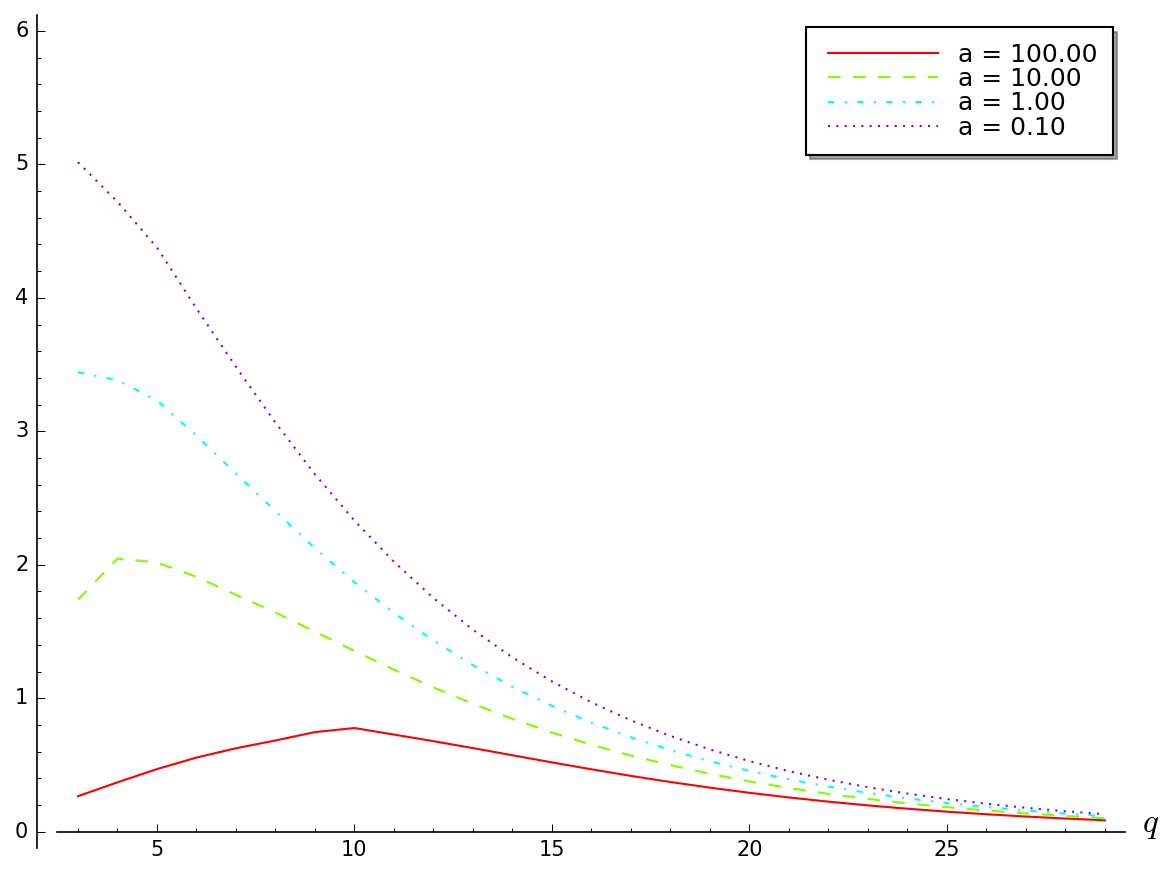
\includegraphics[width=0.8\textwidth]{plots_converging.png}
  \caption
   {
   Зависимость результата численного интегрирования выражения \ref{eq:split} при различных ненулевых $a$, где $r = 1 - 2^{-q}$. Можно наблюдать тенденцию к сходимости интегралов.
   }\label{fig:ring_convergence}
\end{figure}

\begin{figure}[ht]
  \centering
  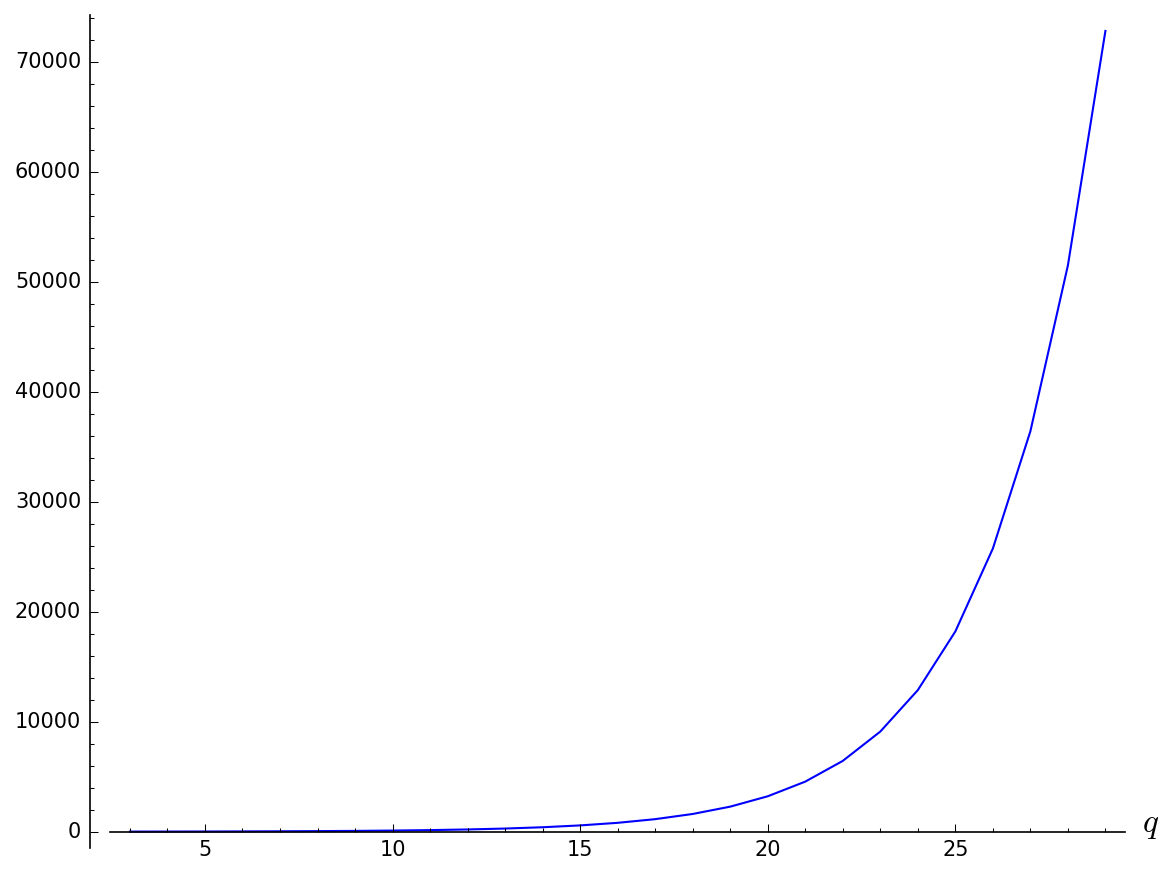
\includegraphics[width=0.8\textwidth]{plots_diverging.png}
  \caption
   {
   Зависимость результата численного интегрирования выражения \ref{eq:split} при $a = 0$, где $r = 1 - 2^{-q}$. Можно наблюдать тенденцию к расходимости интеграла.
   }\label{fig:ring_divergence}
\end{figure}

Можно интуитивно обосновать, почему интеграл сходится. Рассмотрим $\det S(\iu y)$ при большом $y$, в этому случае получаем:
\begin{align*}
\det S(\iu y)
&= 
\frac
{\eexp{\iu \iu y} + \frac{a}{2 \iu y} \frac{\eexp{\iu \iu y} + \eexp{-\iu \iu y}}{2\iu} - 1}
{\eexp{-\iu \iu y} + \frac{a}{2 \iu y} \frac{\eexp{\iu \iu y} + \eexp{-\iu \iu y}}{2\iu} - 1}
\\ &=
\frac
{\eexp{- y} - \frac{a}{4 y} (\eexp{- y} + \eexp{y}) - 1}
{\eexp{y} - \frac{a}{4 y}  (\eexp{- y} + \eexp{y}) - 1}
\end{align*}
, так как $e^{-y} \to 0$, $y e^{-y} \to 0$, легко видеть, что выражение выше будет иметь порядок $\frac{a}{y}$, и, соответственно, его логарифм — порядок $\ln y$, что является принципиальным отличием от случая $a=0$, когда порядок логарифма был $y$ (см. \autoref{sec:ring_incompl_proof}). Однако, строгое обоснование данного факта требует более тщательного анализа.
